\chapter{Realisierung}

\section{Systemübersicht}

\begin{figure}[H]
	\centering
	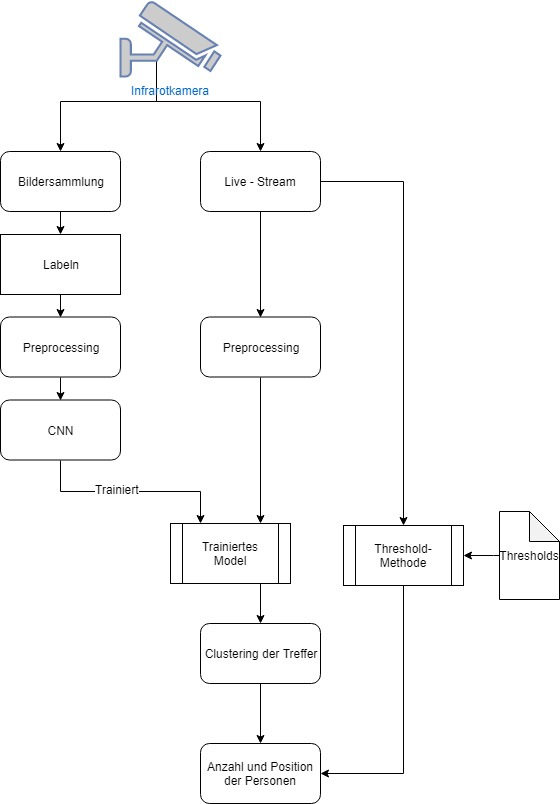
\includegraphics[width=.8\linewidth]{SystemOverview}
	\caption{Grobübersicht des Systems mit CNN- und Thresholdalgorithmus}
	\label{SystemOverview}
\end{figure}

\section{UDP-Schnittstelle}

Um die Bilder automatisiert erhalten zu können wurde eine Schnittstelle zu den Infrarotkameras implementiert. Es wurde das UDP-Protokoll verwendet, da die Kameras nur über dieses Protokoll angesprochen werden konnten.\\
 Die einzige ander Möglichkeit and Bilder zu gelangen wäre über die GUI Applikation des Herstellers Videos aufzunehmen. Dies sind bereits auf RGB convertiert, beihalten also nicht alle Information des ursprünglichen Bildes und die Applikation kann nicht automatisiert angesprochen werden. Folglich ist dies keine praktikable Variante um effizient Daten zu sammeln.\\
\\
Die Kameras können ausserdem nur mittels UDP-Broadcasts identifiziert und and einen Socket gebunden werden. Aus diesem Grund konnten die Kameras nicht im allgemeinen Schulnetzwerk installiert werden, sondern mussten in einem separaten Netzwerk betrieben werden. In diesem Netzwerk konnten sie über einen Computer angesteuert werden, der widerum mit dem HSLU-Netzwerk verbunden ist. Um die Entwicklung der Schnittstelle möglichst einfach zu gestalten wurde versucht einen Remoteinterpreter aufzusetzen. Dies ist eine funktion von Pycharm \parencite{bibid} erlaubt es, auf einem Lokalen system zu entwickeln aber die Software direkt auf einem Remote System auszuführen und zu Debuggen.\\
Leider wird dies von 

\subsection{Interne Schnittstellen}


\subsection{Umsetzung Programmierung}

\subsection{Testing}
